% ----------------------------------------------------------------------------
% DSP
% ----------------------------------------------------------------------------

\chapter{Processamento de Sinais Digitais}

\todo{Precisa mudar o nome dos exemplos para exemplo~. Neste caso, a função setup deve ser renomeada para "tilde\_setup")}

Enfim chegamos no processamento de áudio propriamente dito: \emph{Digital
Signal Processing} ou processamento de sinal digital. O Pure Data possui
inlets e outlets específicos para o processamento de sinal. É fácil
reconhecer: eles são pintados de cinza escuro.

\begin{figure}[h!]
\centering
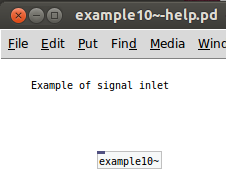
\includegraphics[width=0.7\textwidth]{example10}
\caption{Primeiro Inlet DSP}
\end{figure}

\section{Primeiro inlet para DSP}

Para realizar DSP no Pure Data é necessário alguns cuidados (veja o exemplo
10). Primeiramente, é necessário possuir na estrutura de dados um atributo do
tipo \texttt{t\_float} para armazenar o valor de entrada do inlet.

\lstinputlisting[name=Exemplo 10,linerange=6-9]{../examples/src/example10.c}

Se o \external necessita de apenas um inlet DSP, a macro
\texttt{CLASS\_MAINSIGNALIN()} define um inlet DSP no primeiro inlet da
esquerda. Para esta macro funcionar, é necessário que a classe seja do tipo
\texttt{CLASS\_DEFAULT}, e que um método seja associado à mensagem ``dsp", de
forma que será executado qunado o DSP for iniciado. A forma de declaração de
outros inlets DSP será vista logo adiante.

\lstinputlisting[name=Exemplo 10,linerange=36-49,firstnumber=last]{../examples/src/example10.c}
 
O próximo passo é definir o método DSP que associamos na função
\texttt{\_setup()}:

\lstinputlisting[name=Exemplo 10,linerange=31-34,firstnumber=last]{../examples/src/example10.c}

Todo método de processamento de sinais associado através da função
\texttt{dsp\_add()} será executado em todo ciclo DSP enquanto o processamento
de sinais estiver ligado para o Pure Data ou para aquela janela específica,
através do objeto \texttt{switch~}. Por isto, cuidado com alocações de
memória, inicialização de variáveis, etc.

Neste exemplo, o método \texttt{example10\_perform()} é associado ao
processamento de áudio do Pure Data e será chamada em cada execução do ciclo
DSP com 3 argumentos: o endereço para o sinal de entrada
(\texttt{sp[0]->s\_vec}), a quantidade de amostras no bloco
(\texttt{sp[0]->s\_n}), e o endereço da estrutura que contém sua instância
(\texttt{x}).

Podemos passar para o método perform quaisquer parâmetros em qualquer ordem.
Só é importante e óbvio que devemos lembrar quais parâmetros foram passados e
em qual ordem. O próximo passo é criar o método perform propriamente dito.

\lstinputlisting[name=Exemplo 10,linerange=23-29,firstnumber=last]{../examples/src/example10.c}

\todo{O que raios há na posição w[0]? Resposta: o endereço da própria função
perform.}

O método perform receberá como parâmetro um vetor com os valores definidos no
método \texttt{dsp\_add()}. A posição 0 deste vetor sempre conterá o endereço
para a própria função \texttt{\_perform()}. Na posição 1, o sinal de entrada;
na posição 2 o tamanho do vetor de entrada e na posição 3 a estrutura de dados
correspondente ao objeto. Este método deve retornar a próxima posição do
vetor, ou seja, o endereço dado na chamada somado com a quantidade de
atributos do método mais um.

\section{Vários inlets DSP}

É possível definir vários inlets de DSP para um \external (veja o exemplo 11).
A criação de inlets adicionais não é feita no método \texttt{\_setup()} mas
sim no construtor do objeto. Quanto ao primeiro inlet, só é necessário
definí-lo explicitamnete no construtor se a classe não for do tipo
\texttt{CLASS\_DEFAULT}.

\lstinputlisting[name=Exemplo 11,linerange=12-19]{../examples/src/example11.c}

Neste caso, a utilização do método \texttt{class\_addmethod} é exatamente
igual à anterior, a menos de uma mudança na quantidade de parâmetros por causa
da quantidade de inlets:

\lstinputlisting[name=Exemplo 11,linerange=36-38,firstnumber=last]{../examples/src/example11.c}

Note que precisamos agora alterar a quantidade de parâmetros passadas ao método
\texttt{\_perform()}, que ficará assim:

\lstinputlisting[name=Exemplo 11,linerange=26-34,firstnumber=last]{../examples/src/example11.c}

Neste ponto, este external deve ter uma aparência como na figura
\ref{fig:inlets-dsp}.

\begin{figure}[h!]
\centering
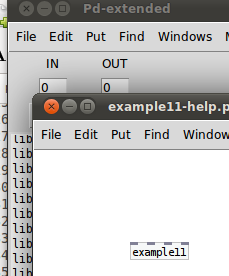
\includegraphics[width=0.3\textwidth]{example11}
\caption{Vários inlets DSP.}
\label{fig:inlets-dsp}
\end{figure}

\section{Primeiro outlet DSP}

A criação dos outlets é feita no construtor do external (veja o exemplo 12) e
não é necessário adicionar os outlets à estrutura da classe.

\lstinputlisting[name=Exemplo 12,linerange=12-20]{../examples/src/example12.c}

A definição do método \texttt{\_perform()} será idêntica ao do exemplo
anterior, quando criamos quatro inlets:

\lstinputlisting[name=Exemplo 12,linerange=37-39,firstnumber=last]{../examples/src/example12.c}

O método perform também será quase idêntico ao do exemplo anterior, porém
recebendo quatro outlets:

\lstinputlisting[name=Exemplo 12,linerange=27-35,firstnumber=last]{../examples/src/example12.c}

O resultado pode ser visto na figura \ref{fig:primeiro-outlet}.

\begin{figure}[h!]
\centering
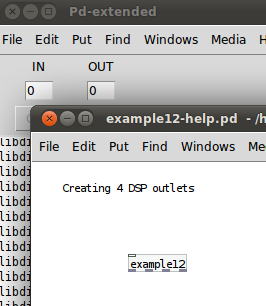
\includegraphics[width=0.3\textwidth]{example12}
\caption{Primeiro Outlet DSP.}
\label{fig:primeiro-outlet}
\end{figure}

\section{Inlets e outlets DSP}

Nosso próximo exemplo (veja o exemplo 13) mistura no mesmo objeto inlets e
outlets DSP, o que é bastante comum. Neste ponto, deve estar mais ou menos
claro como é feita a construção de um objeto assim. Lembre-se que não é
necessário guardar os endereços dos inlets e outlets na estrutura de dados que
representa o objeto. É necessário apenas criar os inlets e outlets no
construtor (lembre-se que o primeiro inlet já foi criado no método setup. Ele
é mágico!).

\lstinputlisting[name=Exemplo 13,linerange=12-25]{../examples/src/example13.c}

No método seguinte associamos o método \texttt{\_perform()} à cadeia DSP do
Pure Data:

\lstinputlisting[name=Exemplo 13,linerange=46-48,firstnumber=last]{../examples/src/example13.c}

No método \texttt{\_perform()} recebemos como argumento um bloco de memória
que contém primeiro os buffers de entrada e em seguida os buffers de saída:

\lstinputlisting[name=Exemplo 13,linerange=32-44,firstnumber=last]{../examples/src/example13.c}

O resultado pode ser visto na figura \ref{fig:varios-inlets-outlets}.

\begin{figure}[h!]
\centering
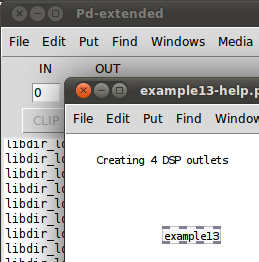
\includegraphics[width=0.3\textwidth]{example13}
\caption{Vários inlets e outlets DSP.}
\label{fig:varios-inlets-outlets}
\end{figure}

\section{Inlets e outlets DSP criados dinamicamente}

É possível definir através de parâmetros para o construtor a quantidade de
inlets e/ou outlets DSP que um external deve possuir. Isso significa que o
número de inlets e outlets é definido dinamicamente, em tempo de execução,
através de um argumento. Para isto, existe mais de uma possibilidade de
implementação.

A primeira possibilidade consiste em passarmos para o construtor a informação
de quantos inlets e outlets teremos na função dsp (veja o exemplo
17) e armazenarmos na estrutura de dados que contém o objeto do \external.

\lstinputlisting[name=Exemplo 17,linerange=6-25]{../examples/src/example17.c}

Na passagem de parâmetro para o DSP usamos estas variáveis para contar quantos
parâmetros serão usados.

\lstinputlisting[name=Exemplo 17,linerange=33-48,firstnumber=last]{../examples/src/example17.c}

A segunda opção é usar outro método que baseia-se no modelo de alocação de
memória do pd. Criamos um vetor e apontamos este vetor para o dado da entrada
/ saída do external. Assim podemos utilizar a estrutura amarrada ao external
para produzir / consumir o dado. Veja o exemplo 19.

\lstinputlisting[name=Exemplo 19,linerange=45-54]{../examples/src/example19.c}

Neste ponto, esta solução é bastante parecida com a anterior e poderia ser usada também com uma quantidade
variável de outlets. A alteração está na estrutura da classe.

\lstinputlisting[name=Exemplo 19,linerange=6-10,firstnumber=last]{../examples/src/example19.c}

Ok, 64 não é um número mágico de verdade. Ele é o tamanho de bloco padrão do
Pure Data. Para que esta solução seja genérica o suficiente é melhor usar a
função \texttt{sys\_getblksize()} para obter o tamanho do bloco e alocar
a quantidade correta de espaço. Da forma em que está, corremos o risco de
obter erros de leitura ou escrita em lugares sem permissão. 

\lstinputlisting[name=Exemplo 19,linerange=14-22,firstnumber=last]{../examples/src/example19.c}

Como no exemplo anterior, o construtor cria a quantidade de outlets passada
como argumento na criação do objeto. Aqui, poderíamos utilizar
\texttt{malloc()} para alocar o vetor com os dados de maneira inteligente ao
invés de usar o 64 mágico.

\lstinputlisting[name=Exemplo 19,linerange=36-41,firstnumber=last]{../examples/src/example19.c}

O método DSP não fará mais que passar o próprio objeto ao método
\texttt{\_perform()}. Na verdade, poderia não passar nem o objeto.

\lstinputlisting[name=Exemplo 19,linerange=30-34,firstnumber=last]{../examples/src/example19.c}

A função perform não precisa fazer nada mais que despertar o processo
consumidor e liberar o processamento no Pure Data. E este é um ponto que
considero importante para levantar outro questionamento.

O Pd precisa que o processamento dos blocos termine em determinado tempo. Qual
seria este tempo? Para um bloco de 64 amostras e taxa de amostragem 44.100
amostras por segundo, é necessário que todo o processamento para um bloco
termine em um pouco mais de 1 milisegundo. Parece rápido mas seu computador é
mais rápido que isto. Criar um processo consumidor e fazê-lo liberando
\todo{``fazê-lo liberando"?} o bloco de processamento pode ser uma abordagem
melhor para processos baseados em fluxo, como escrita em arquivos. Para isto
precisamos utilizar outra função em outra thread e este é nosso próximo
assunto.

\todo{Vale a pena mostrar como fazer o loop entre as amostras ou é óbvio?}
